\chapter{Huracán Katrina} \label{cap0b}
%\addcontentsline{toc}{chapter}{Huracán Katrina}

\begin{flushright}
\begin{minipage}{7.85cm}
    {\em blbalbalbal} \\ Alguien %TODO
\end{minipage}
\end{flushright}

\vspace*{5mm}

\section{Introducción}

El huracán Katrina fue uno de los ciclones tropicales más mortíferos,
destructivos y costosos que haya impactado a Estados Unidos en décadas. Katrina
formó parte de la Temporada de huracanes en el Atlántico de 2005. Fue la tercera
tormenta más poderosa de la temporada.

\begin{figure}[H]
 \centering
 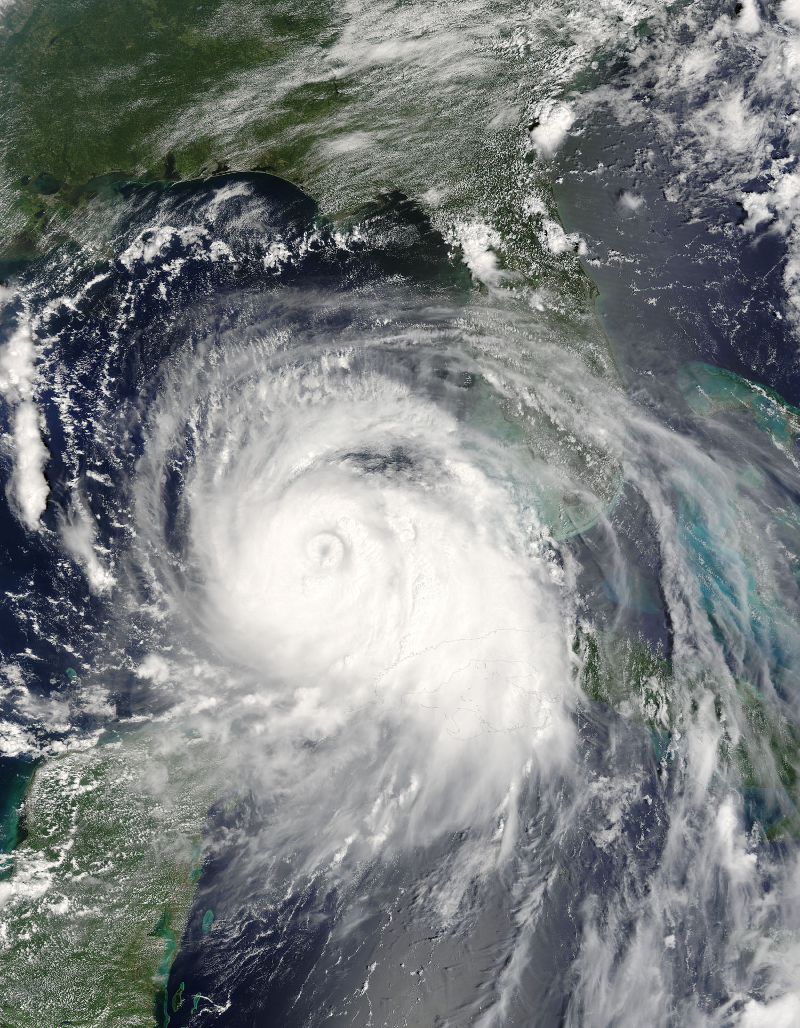
\includegraphics[width=120mm]{figuras/cap0/hurricane.png}
 \caption{Huracán Katrina visto desde el espacio}
\end{figure}

Fue un gran ciclón tropical que azotó el sur y el centro de los Estados Unidos
en agosto de 2005. Produjo grandes destrozos en Florida, Bahamas, Luisiana y
Misisipi, incluyendo cuantiosos daños materiales y graves inundaciones.

\begin{figure}[H]
 \centering
 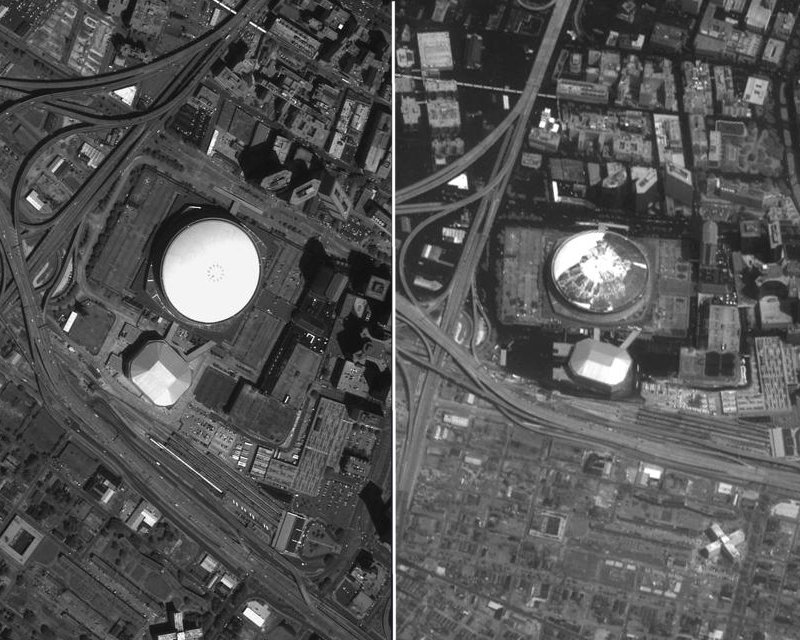
\includegraphics[width=120mm]{figuras/cap0/before_after.png}
 \caption{Daños producidos por el huracán al {\em Superdome}}
\end{figure}

Tocó tierra en la costa de Luisiana el 29 de agosto convertido en un huracán
categoría 3, y a pesar de que en el último momento se desvió ligeramente de su
ruta, que atravesaba directamente la ciudad de Nueva Orleans, se produjo una
gran devastación en la misma y en zonas cercanas. Por los daños producidos, se
convirtió en uno de los huracanes más devastadores en Estados Unidos en la
historia reciente, y quizás sea el mayor desastre natural en la historia de ese
país.

Se estima que el Katrina causó daños materiales por 75 mil millones de dólares
estadounidenses, convirtiéndose en el huracán más costoso en la historia de los
Estados Unidos; la tormenta causó la muerte a 1.836 personas, convirtiéndose en
el huracán más mortífero de Estados Unidos desde el Huracán Okeechobee de 1928.

\subsection{Nueva Orleans}

El 2 de septiembre de 2005 el 85\% de la ciudad de Nueva Orleans estaba bajo el
agua, donde en algunas zonas llegó a 7 m de profundidad. Durante un tiempo, la
ciudad estuvo inhabitable. Todos los servicios públicos estaban suspendidos y no
era posible utilizar la infraestructura física debido a la gran cantidad de
agua. Además está en crisis de orden público debido al violento saqueo
generalizado que se presenta por la falta de alimentos y servicios públicos. El
Superdome, principal refugio "de última hora" ya empezó a ser evacuado debido al
deterioro de las condiciones de vida en su interior (amenaza a los generadores,
falta de aire acondicionado e interrupción del servicio de acueducto).

Los días y 1 de septiembre se generalizó el vandalismo y la escasez de
alimentos, vivienda y agua produjo un desorden civil de grandes proporciones. La
tarde del 1 de septiembre, la oficina del alcalde pidió ayuda urgente para
controlar la situación que ha alcanzado niveles desmedidos\footnote{Fox News
``AtroDrome no puede acoger más refugiados'' :
\url{http://www.foxnews.com/story/0,2933,168112,00.html}}. Durante varios días
estuvo vigente la ley marcial, el uso de la fuerza contra el saqueo y la
recomendación urgente de abandonar la ciudad a través de la conexión con
Crescent City, o en su defecto buscar refugio en pisos más altos. La rotura de
una sección del dique hizo que el nivel de agua aumentase en vez de disminuir, y
los esfuerzos para reconstruirlo temporalmente arrojando bolsas de arena desde
helicópteros no resultaron efectivos. De acuerdo con la cadena de noticias Fox
News, en la tarde del 30 de agosto, y en atención a la imposibilidad de
restaurar el aislamiento con el lago Pontchartrain, y al empeoramiento de las
condiciones de vida en los albergues, la gobernadora de Luisiana, Kathleen
Blanco, ordenó la evacuación de todos los residentes de Nueva Orleans.

%%% Local Variables:
%%% mode: latex
%%% TeX-master: "../dissim"
%%% End: